\documentclass[12pt, a4paper]{article}

%<*preamble>
% Math symbols
\usepackage{amsmath, amsthm, amsfonts, amssymb}
\usepackage{accents}
\usepackage{esvect}
\usepackage{mathrsfs}
\usepackage{mathtools}
\mathtoolsset{showonlyrefs}
\usepackage{cmll}
\usepackage{stmaryrd}
\usepackage{physics}
\usepackage[normalem]{ulem}
\usepackage{ebproof}
\usepackage{extarrows}

% Page layout
\usepackage{geometry, a4wide, parskip, fancyhdr}

% Font, encoding, russian support
\usepackage[russian]{babel}
\usepackage[sb]{libertine}
\usepackage{xltxtra}

% Listings
\usepackage{listings}
\lstset{basicstyle=\ttfamily,breaklines=true}
\setmonofont{Inconsolata}

% Miscellaneous
\usepackage{array}
\usepackage{calc}
\usepackage{caption}
\usepackage{subcaption}
\captionsetup{justification=centering,margin=2cm}
\usepackage{catchfilebetweentags}
\usepackage{enumitem}
\usepackage{etoolbox}
\usepackage{float}
\usepackage{lastpage}
\usepackage{minted}
\usepackage{svg}
\usepackage{wrapfig}
\usepackage{xcolor}
\usepackage[makeroom]{cancel}

\newcolumntype{L}{>{$}l<{$}}
    \newcolumntype{C}{>{$}c<{$}}
\newcolumntype{R}{>{$}r<{$}}

% Footnotes
\usepackage[hang]{footmisc}
\setlength{\footnotemargin}{2mm}
\makeatletter
\def\blfootnote{\gdef\@thefnmark{}\@footnotetext}
\makeatother

% References
\usepackage{hyperref}
\hypersetup{
    colorlinks,
    linkcolor={blue!80!black},
    citecolor={blue!80!black},
    urlcolor={blue!80!black},
}

% tikz
\usepackage{tikz}
\usepackage{tikz-cd}
\usetikzlibrary{arrows.meta}
\usetikzlibrary{decorations.pathmorphing}
\usetikzlibrary{calc}
\usetikzlibrary{patterns}
\usepackage{pgfplots}
\pgfplotsset{width=10cm,compat=1.9}
\newcommand\irregularcircle[2]{% radius, irregularity
    \pgfextra {\pgfmathsetmacro\len{(#1)+rand*(#2)}}
    +(0:\len pt)
    \foreach \a in {10,20,...,350}{
            \pgfextra {\pgfmathsetmacro\len{(#1)+rand*(#2)}}
            -- +(\a:\len pt)
        } -- cycle
}

\providetoggle{useproofs}
\settoggle{useproofs}{false}

\pagestyle{fancy}
\lfoot{M3137y2019}
\cfoot{}
\rhead{стр. \thepage\ из \pageref*{LastPage}}

\newcommand{\R}{\mathbb{R}}
\newcommand{\Q}{\mathbb{Q}}
\newcommand{\Z}{\mathbb{Z}}
\newcommand{\B}{\mathbb{B}}
\newcommand{\N}{\mathbb{N}}
\renewcommand{\Re}{\mathfrak{R}}
\renewcommand{\Im}{\mathfrak{I}}

\newcommand{\const}{\text{const}}
\newcommand{\cond}{\text{cond}}

\newcommand{\teormin}{\textcolor{red}{!}\ }

\DeclareMathOperator*{\xor}{\oplus}
\DeclareMathOperator*{\equ}{\sim}
\DeclareMathOperator{\sign}{\text{sign}}
\DeclareMathOperator{\Sym}{\text{Sym}}
\DeclareMathOperator{\Asym}{\text{Asym}}

\DeclarePairedDelimiter{\ceil}{\lceil}{\rceil}

% godel
\newbox\gnBoxA
\newdimen\gnCornerHgt
\setbox\gnBoxA=\hbox{$\ulcorner$}
\global\gnCornerHgt=\ht\gnBoxA
\newdimen\gnArgHgt
\def\godel #1{%
    \setbox\gnBoxA=\hbox{$#1$}%
    \gnArgHgt=\ht\gnBoxA%
    \ifnum     \gnArgHgt<\gnCornerHgt \gnArgHgt=0pt%
    \else \advance \gnArgHgt by -\gnCornerHgt%
    \fi \raise\gnArgHgt\hbox{$\ulcorner$} \box\gnBoxA %
    \raise\gnArgHgt\hbox{$\urcorner$}}

% \theoremstyle{plain}

\theoremstyle{definition}
\newtheorem{theorem}{Теорема}
\newtheorem*{definition}{Определение}
\newtheorem{axiom}{Аксиома}
\newtheorem*{axiom*}{Аксиома}
\newtheorem{lemma}{Лемма}

\theoremstyle{remark}
\newtheorem*{remark}{Примечание}
\newtheorem*{exercise}{Упражнение}
\newtheorem{corollary}{Следствие}[theorem]
\newtheorem*{statement}{Утверждение}
\newtheorem*{corollary*}{Следствие}
\newtheorem*{example}{Пример}
\newtheorem{observation}{Наблюдение}
\newtheorem*{prop}{Свойства}
\newtheorem*{obozn}{Обозначение}

% subtheorem
\makeatletter
\newenvironment{subtheorem}[1]{%
    \def\subtheoremcounter{#1}%
    \refstepcounter{#1}%
    \protected@edef\theparentnumber{\csname the#1\endcsname}%
    \setcounter{parentnumber}{\value{#1}}%
    \setcounter{#1}{0}%
    \expandafter\def\csname the#1\endcsname{\theparentnumber.\Alph{#1}}%
    \ignorespaces
}{%
    \setcounter{\subtheoremcounter}{\value{parentnumber}}%
    \ignorespacesafterend
}
\makeatother
\newcounter{parentnumber}

\newtheorem{manualtheoreminner}{Теорема}
\newenvironment{manualtheorem}[1]{%
    \renewcommand\themanualtheoreminner{#1}%
    \manualtheoreminner
}{\endmanualtheoreminner}

\newcommand{\dbltilde}[1]{\accentset{\approx}{#1}}
\newcommand{\intt}{\int\!}

% magical thing that fixes paragraphs
\makeatletter
\patchcmd{\CatchFBT@Fin@l}{\endlinechar\m@ne}{}
{}{\typeout{Unsuccessful patch!}}
\makeatother

\newcommand{\get}[2]{
    \ExecuteMetaData[#1]{#2}
}

\newcommand{\getproof}[2]{
    \iftoggle{useproofs}{\ExecuteMetaData[#1]{#2proof}}{}
}

\newcommand{\getwithproof}[2]{
    \get{#1}{#2}
    \getproof{#1}{#2}
}

\newcommand{\import}[3]{
    \subsection{#1}
    \getwithproof{#2}{#3}
}

\newcommand{\given}[1]{
    Дано выше. (\ref{#1}, стр. \pageref{#1})
}

\renewcommand{\ker}{\text{Ker }}
\newcommand{\im}{\text{Im }}
\renewcommand{\grad}{\text{grad}}
\newcommand{\rg}{\text{rg}}
\newcommand{\defeq}{\stackrel{\text{def}}{=}}
\newcommand{\defeqfor}[1]{\stackrel{\text{def } #1}{=}}
\newcommand{\itemfix}{\leavevmode\makeatletter\makeatother}
\newcommand{\?}{\textcolor{red}{???}}
\renewcommand{\emptyset}{\varnothing}
\newcommand{\longarrow}[1]{\xRightarrow[#1]{\qquad}}
\DeclareMathOperator*{\esup}{\text{ess sup}}
\newcommand\smallO{
    \mathchoice
    {{\scriptstyle\mathcal{O}}}% \displaystyle
    {{\scriptstyle\mathcal{O}}}% \textstyle
    {{\scriptscriptstyle\mathcal{O}}}% \scriptstyle
    {\scalebox{.6}{$\scriptscriptstyle\mathcal{O}$}}%\scriptscriptstyle
}
\renewcommand{\div}{\text{div}\ }
\newcommand{\rot}{\text{rot}\ }
\newcommand{\cov}{\text{cov}}

\makeatletter
\newcommand{\oplabel}[1]{\refstepcounter{equation}(\theequation\ltx@label{#1})}
\makeatother

\newcommand{\symref}[2]{\stackrel{\oplabel{#1}}{#2}}
\newcommand{\symrefeq}[1]{\symref{#1}{=}}

% xrightrightarrows
\makeatletter
\newcommand*{\relrelbarsep}{.386ex}
\newcommand*{\relrelbar}{%
    \mathrel{%
        \mathpalette\@relrelbar\relrelbarsep
    }%
}
\newcommand*{\@relrelbar}[2]{%
    \raise#2\hbox to 0pt{$\m@th#1\relbar$\hss}%
    \lower#2\hbox{$\m@th#1\relbar$}%
}
\providecommand*{\rightrightarrowsfill@}{%
    \arrowfill@\relrelbar\relrelbar\rightrightarrows
}
\providecommand*{\leftleftarrowsfill@}{%
    \arrowfill@\leftleftarrows\relrelbar\relrelbar
}
\providecommand*{\xrightrightarrows}[2][]{%
    \ext@arrow 0359\rightrightarrowsfill@{#1}{#2}%
}
\providecommand*{\xleftleftarrows}[2][]{%
    \ext@arrow 3095\leftleftarrowsfill@{#1}{#2}%
}

\allowdisplaybreaks

\newcommand{\unfinished}{\textcolor{red}{Не дописано}}

% Reproducible pdf builds 
\special{pdf:trailerid [
<00112233445566778899aabbccddeeff>
<00112233445566778899aabbccddeeff>
]}
%</preamble>


\lhead{Математический анализ}
\cfoot{}
\rfoot{21.12.2020}

\begin{document}

\begin{corollary}[из 5 свойства меры Лебега]
    \(\forall A\in \mathfrak{M}^m\ \ \exists B,C\) --- борелевские:
    \[B\subset A\subset C \quad \lambda(C\setminus A) = 0, \lambda(A\setminus B) = 0\]
\end{corollary}
\begin{proof}
    \[C: = \bigcap_{n = 1}^{+\infty} G_{\frac{1}{n}} \quad B \subset \bigcup_{n = 1}^{+\infty} F_{\frac{1}{n}}\]
\end{proof}
\begin{corollary}
    \(\forall A\in \mathfrak{M}^m \ \ \exists B, \mathcal{N} : B\) --- борелевское, \(\mathcal{N}\in \mathfrak{M}^m, \lambda \mathcal{N} = 0\).

    Тогда \(A = B \cup \mathcal{N}\)
\end{corollary}
\begin{proof}
    \(\exists B\) из следствия 1, \(\mathcal{N} : = A\setminus B\)
\end{proof}

\begin{remark}
    Обозначим \(|X|\) --- мощность множества \(X\).

    \[\forall X \ \ |2^X| > |X|\]
    \[|2^{\R^m}| > \text{континуум}\]
    \[\mathcal{B} \subset 2^{\R^m} \text{ --- борелевская \(\sigma\)-алгебра} \ \ |\mathcal{B}| = \text{континуум}\]
    \[\mathfrak{M}^m > \text{континуум}\]
    \(\mathcal{K}\) --- Канторово множество, тогда \(|\mathcal{K}|=\) континуум, \(\lambda \mathcal{K} = 0\)
    \[\forall D\subset \mathcal{K}\ \ D\in \mathfrak{M}^m, \lambda D = 0 \ \ 2^{\mathcal{K}} \subset \mathfrak{M}^m\]
\end{remark}

\begin{corollary}
    \(\forall A\in \mathfrak{M}^m\)
    \[\lambda A = \inf_{\substack{G:A\subset G\\ G \text{ --- откр.}}} \lambda(G) = \sup_{\substack{F:F\subset A\\ F \text{ --- замкн.}}} \lambda(F) \stackrel{(*)}{=} \sup_{\substack{K:K\subset A\\ K \text{ --- комп.}}} \lambda(K)\]
\end{corollary}
\begin{proof}
    \((*)\) следует из \(\sigma\)-конечности \(\R^m = \bigcup\limits_{n = 1}^{+\infty} Q(0, n)\), где \(Q(a, R) = \times_{i = 1}^n [a_i - R, a_i + R]\) --- куб с центром в \(a\) и ребром \(R\).

    \(\lambda(A\cap Q(0, n)) \to \lambda A\) по непрерывности снизу, т.к. \(A\cap Q(0, n)\) хорошо аппроксимируется замкнутым множеством.
\end{proof}

\begin{definition}
    Свойства из следствия 3 называются \textbf{регулярностью} меры Лебега.
\end{definition}

\section*{Преобразование меры Лебега при сдвигах и линейных отображениях}

\begin{lemma}\itemfix
    \begin{itemize}
        \item \((X', \mathfrak{A}', \mu')\) --- пространство с мерой.
        \item \((X, \mathfrak{A}, \_)\) --- ``заготовка'' пространства с мерой
        \item \(\exists T : X \to X'\) --- биекция; \(\forall A\in \mathfrak{A}\ \ TA\in \mathfrak{A}'\) и \(T\text{\O} = \text{\O}\)
    \end{itemize}

    Положим \(\mu A = \mu'(TA)\). Тогда \(\mu\) --- мера.
\end{lemma}
\begin{proof}
    Проверим счётную аддитивность \(\mu\) : \(A = \bigsqcup A_i\)
    \[\mu A = \mu'(TA) = \mu'\left(\bigsqcup TA_i\right) = \sum \mu'(TA_i) = \sum \mu A_i\]
\end{proof}

\begin{lemma}\itemfix
    \begin{itemize}
        \item \(T : \R^m \to \R^n\) --- непр.
        \item \(\forall E\in \mathfrak{M}^m : \lambda E = 0\) выполняется \(\lambda TE = 0\)
    \end{itemize}
    Тогда \(\forall A\in \mathfrak{M}^m \ \ TA\in \mathfrak{M}^m\)
\end{lemma}
\begin{proof}
    \[A = \bigcup_{j = 1}^{+\infty} K_j\cup \mathcal{N}\]
    , где \(K_j\) --- компакт, \(\lambda \mathcal{N} = 0\)
    \[TA = \bigcup_{j = 1}^{+\infty} TK_j \cup T\mathcal{N}\]
    \(TK_j\) компакт как образ компакта при непрерывном отображении. \(\Rightarrow TA\) измеримо.
\end{proof}

\begin{example}[Канторова лестница]
    \begin{figure}[h]
        \centering
        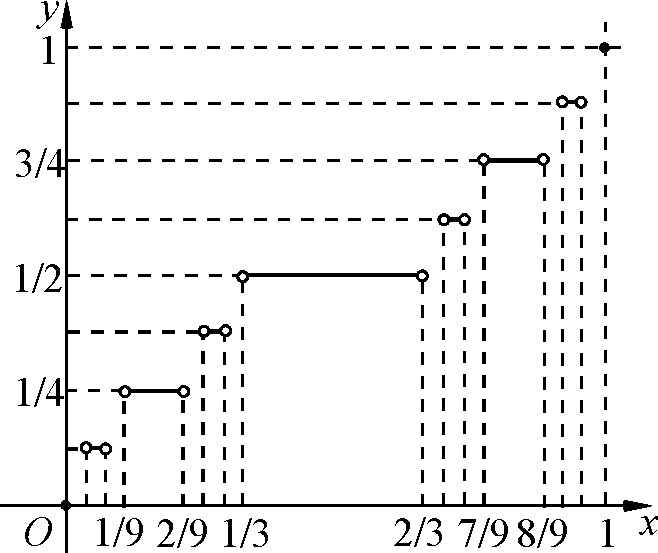
\includegraphics[scale=0.5]{images/cantor_ladder.png}
    \end{figure}
    \[\Delta = [0, 1]\]
    \[\Delta_0 = \left[0, \frac{1}{3}\right] \quad \Delta_1 = \left[\frac{2}{3}, 1\right]\]
    \[\Delta_{00} = \left[0, \frac{1}{9}\right] \quad \Delta_{01} = \left[\frac{2}{9}, \frac{1}{3}\right], \Delta_{10} = \dots, \Delta_{11} = \dots \]
    \begin{align*}
        \mathcal{K}_0 & = \Delta                                                                                               \\
        \mathcal{K}_1 & = \Delta_0\cup \Delta_1                                                                                \\
        \mathcal{K}_2 & = \Delta_{00}\cup \Delta_{01}\cup \Delta_{10}\cup \Delta_{11}                                          \\
                      & \vdots                                                                                                 \\
        \mathcal{K}_n & = \bigcup_{\varepsilon_1 \dots \varepsilon_n \in \{0, 1\} } \Delta_{\varepsilon_1 \dots \varepsilon_n}
    \end{align*}
    \[\mathcal{K} : = \bigcap \mathcal{K}_n\]
    \[f(x) = \begin{cases}
            \frac{1}{2} & , x\in \Delta\setminus \mathcal{K}_1   \\
            \frac{1}{4} & , x\in \Delta_0\setminus \mathcal{K}_2 \\
            \frac{3}{4} & , x\in \Delta_1\setminus \mathcal{K}_2 \\
            \vdots                                               \\
            \sup f(t)   & , t \leq x, t\not\in \mathcal{K}
        \end{cases}\]

    \(f([0, 1]\setminus \mathcal{K}\) --- счётное = множество двоично-рациональных чисел из \([0, 1]\)

    \(\lambda f([0, 1]\setminus \mathcal{K}) = 0\)

    \(\lambda f(\mathcal{K}) = 1\), т.к. \(\forall y\in [0, 1] \ \ \exists x : f(x) = y\), при этом \(f\) непрерывна, т.к. она --- сюръекция.

    Тогда пусть \(E\subset [0, 1]\not\in \mathfrak{M}^m\) : \(f^{ - 1}(E)\) --- подмножество \(\mathcal{K}\) и промежутки --- прообразы двоично рациональных точек \(\in E\), при этом это множество измеримо, т.к. \(\lambda \mathcal{K} = 0\)

    Ещё наблюдение: \(x\not\in \mathcal{K} \Rightarrow f\) --- дифференцируема в \(x\) и \(f' = 0\)
\end{example}

\end{document}